%  This is a LaTex file.

%  Homework for the course "AMath 585:  Applied Linear Algebra and Numerical Analysis", 
%  Autumn quarter, 2009, Anne Greenbaum.


%   A latex format for making homework assignments.


\documentclass[letterpaper,12pt]{article}

%          The page format, somewhat wider and taller page than in art12.sty.

\topmargin -0.1in \headsep 0in \textheight 8.9in \footskip 0.6in
\oddsidemargin 0in  \evensidemargin 0in  \textwidth 6.5in
\usepackage{graphicx}
\usepackage{listings}
\usepackage{caption}
\usepackage{subcaption}
\usepackage{color}
\usepackage{float}
\definecolor{keywords}{RGB}{255,0,90}
\definecolor{comments}{RGB}{0,0,113}
\definecolor{red}{RGB}{160,0,0}
\definecolor{green}{RGB}{0,150,0}
\definecolor{codegreen}{rgb}{0,0.6,0}
\definecolor{codegray}{rgb}{0.5,0.5,0.5}
\definecolor{codepurple}{rgb}{0.58,0,0.82}
\definecolor{backcolour}{rgb}{0.95,0.95,0.92}
\definecolor{brown}{rgb}{0.59, 0.29, 0.0}
\definecolor{beaublue}{rgb}{0.74, 0.83, 0.9}
\definecolor{orange}{rgb}{1.0, 0.5, 0.0}
\definecolor{darkslategray}{rgb}{0.18, 0.31, 0.31}
\definecolor{deepblue}{rgb}{0,0,0.5}
\definecolor{deepred}{rgb}{0.6,0,0}
\definecolor{deepgreen}{rgb}{0,0.5,0}
\lstdefinestyle{myMatlabstyle}{
	language=Matlab,
	backgroundcolor=\color{white},   
	commentstyle=\color{codegreen},
	keywordstyle=\color{blue},
	%identifierstyle=\color{brown},
	numberstyle=\tiny\color{codegray},
	stringstyle=\color{orange},
	basicstyle=\footnotesize,
	breakatwhitespace=false,         
	breaklines=true,                 
	captionpos=b,                    
	keepspaces=true,                 
	numbers=left,                    
	numbersep=5pt,                  
	showspaces=false,                
	showstringspaces=false,
	showtabs=false,                  
	tabsize=2
}
\lstdefinestyle{myPythonstyle}{
	language=Python, 
	basicstyle=\ttfamily\small, 
	keywordstyle=\color{blue},
	backgroundcolor=\color{white}, 
	commentstyle=\color{green},
	stringstyle=\color{red},
	showstringspaces=false,
	%identifierstyle=\color{brown},
	breaklines=true, 
}
\lstset{language=Matlab,frame=single}
\lstset{language=Python,frame=single}
\usepackage{amsmath}
\usepackage{epsfig}         % to insert PostScript figures
       % to insert PostScript figures

\begin{document}


%          Definitions of commonly used symbols.



%          The title and header.

\noindent
{\scriptsize AMath 585, Winter 2018} \hfill 

\begin{center}
\large
Assignment 4.
\normalsize

Jithin D. George, No. 1622555
\end{center}

\noindent
Due Monday, Feb. 5.




\begin{enumerate}
\item (finite elements)
Use the Galerkin finite element method with continuous piecewise linear
basis functions to solve the problem
\[
- \frac{d}{dx} \left( (1 + x^2 ) \frac{du}{dx} \right) = f(x) ,~~0 \leq x \leq 1,
\]
\[
u(0) = 0,~~u(1) = 0 .
\]
\begin{enumerate}
\item
Derive the matrix equation that you will need to solve for this problem.

{\bf Solution:}
 \[\hat{u} = \sum_{j=1}^{n-1} c_j \psi_j\]      
        
\[
 \left( \begin{array}{ccccc}

a_{ii} & a_{ii+1}  &    &              \\
 a_{ii-1}  & \ddots & \ddots   &    \\
    & \ddots & \ddots  &\ddots   \\
       &        &  a_{ii-1}     & a_{ii} \end{array} \right)
\left( \begin{array}{c}  c_1 \\ \vdots \\ \vdots \\ c_{n-1}  \end{array} 
\right) =
\left( \begin{array}{c}  \langle f,\psi_1 \rangle \\ \vdots \\  \vdots \\
\langle f, \psi_{n-1} \rangle \end{array} \right) 
\]

\begin{align*}
  a_{ii} &= \int_0^1 (1+x^2) (\psi_i')^2 dx\\
  &= \int_{x_{i-1}}^{x_i} (1+x^2) \frac{1}{(x_i-{x_{i-1}})^2} dx + \int_{x_{i}}^{x_{i+1}} (1+x^2) \frac{1}{(x_{i+1}-{x_{i}})^2} dx\\
 &=  \frac{1}{x_i-{x_{i-1}}} +  \frac{x_i^3-{x_{i-1}^3}}{3(x_i-{x_{i-1}})^2}+\frac{1}{x_{i+1}-{x_{i}}} +  \frac{x_{i+1}^3-{x_{i}^3}}{3(x_{i+1}-{x_{i}})^2}
  \end{align*}
  

  
\begin{align*}
a_{ii-1} &= \int_0^1 (1+x^2) \psi_i \psi_{i-1} dx\\
  &= -\int_{x_{i-1}}^{x_i} (1+x^2) \frac{1}{(x_i-{x_{i-1}})^2} dx \\
 &=  -\frac{1}{x_i-{x_{i-1}}} -  \frac{x_i^3-{x_{i-1}^3}}{3(x_i-{x_{i-1}})^2}
  \end{align*}
  
 \begin{align*}
a_{ii+1} &= \int_0^1 (1+x^2) \psi_i \psi_{i+1} dx\\
 % &=  -\int_{x_{i}}^{x_{i+1}} (1+x^2) \frac{1}{(x_{i+1}-{x_{i}})^2} dx \\
 &=  -\frac{1}{x_{i+1}-{x_{i}}} -  \frac{x_{i+1}^3-{x_{i}^3}}{3(x_{i+1}-{x_{i}})^2}
 \end{align*}
 \[\langle f,\psi_i \rangle =  \int_0^1 f \psi_i dx = \int_{x_{i-1}}^{x_i} f \psi_i dx+ \int_{x_i}^{x_{i+1}} f \psi_i dx \]

 \item
Write a code to solve this set of equations.  You can test your
code on a problem where you know the solution by choosing a function
$u(x)$ that satisfies the boundary conditions and determining what
$f(x)$ must be in order for $u(x)$ to satisfy the differential equation.
Try $u(x) = x(1-x)$.  Then $f(x) = 2(3 x^2 -x + 1)$.

{\bf Solution:}

\begin{figure}[H]

\centering
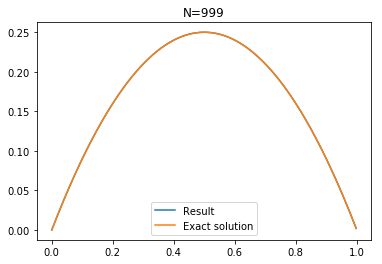
\includegraphics[width=0.5\textwidth]{41.png}



\end{figure}


	\begin{lstlisting}[style=myPythonstyle]
import numpy as np
import matplotlib.pyplot as plt

def f(x):
    return 6*x**2-2*x+2  
def xf(x):
    return 6*x**3-2*x**2+2*x  
def intf(x):
    return 2*x**3-x**2+2*x  
def intxf(x):
    return (6/4)*x**4-(2/3)*x**3+x**2  
def fmaker(x,i):
    return (x[i+1]/(x[i+1]-x[i]))*(intf(x[i+1])-intf(x[i])) - (x[i-1]/(x[i]-x[i-1]))*(intf(x[i])-intf(x[i-1]))+(1/(x[i]-x[i-1]))*(intxf(x[i])-intxf(x[i-1])) -(1/(x[i+1]-x[i]))*(intxf(x[i+1])-intxf(x[i])) 
def aij(x,i):
    return 1/(x[i]-x[i-1]) +(x[i]**3-x[i-1]**3)/(3*(x[i]-x[i-1])**2)
def aii(x,i):
    return aij(x,i)+aij(x,i+1)
def tridiag(a, b, c, k1=-1, k2=0, k3=1):
    return np.diag(a, k1) + np.diag(b, k2) + np.diag(c, k3)
N=1000
x=np.array([])
for i in range(N):
    x= np.append(x,(i/(N-1))**2)
#x=np.linspace(0,1,N)
fe = np.array([])
aiivec = np.array([])
aijvec = np.array([])
for i in range(1,len(x)-1):
    fe=np.append(fe,fmaker(x,i))  
    aiivec =np.append(aiivec,aii(x,i))
    aijvec =np.append(aijvec,-aij(x,i))
mat2=tridiag(aijvec[1:],aiivec,aijvec[1:])
z=np.zeros(N-2)
k = np.linalg.solve(mat2,fe)
y=x[1:-1]
plt.plot(y,k, label = "Result")
exact=y*(1-y)
plt.plot(y,exact, label = "Exact solution")
plt.legend()
print(np.linalg.norm(k-exact, np.inf))
plt.title("N="+str(N))

\end{lstlisting}
\item
Try several different values for the mesh size $h$.  Based on your results,
what would you say is the order of accuracy of the Galerkin method with
continuous piecewise linear basis functions?

{\bf Solution:}

The infinity norm is used here.

\begin{tabular}{rr}
\hline
    h &      Error \\
\hline
 0.01  & 3.2112324338e-06\\
 0.001 & 3.1537675276e-08 \\
\hline
\end{tabular}

The order seems to be O($h^2$)
\item
Now try a nonuniform mesh spacing, say, $x_i = (i/(m+1) )^2$, $i=0,1, \ldots ,
m+1$.  Do you see the same order of accuracy, if $h$ is defined as
the maximum mesh spacing, $\max_i ( x_{i+1} - x_i )$?

{\bf Solution:}

The infinity norm is used here.

\begin{tabular}{rr}
\hline
    h &      Error \\
\hline
 0.02  & 1.23156638885e-05\\
 0.002 & 1.20969674222e-07 \\
\hline
\end{tabular} 

Again, the order seems to be O($h^2$).
\item
Suppose the boundary conditions were $u(0) = a$, $u(1) = b$.  Show how you would
represent the approximate solution $\hat{u} (x)$ as a linear combination of hat
functions and how the matrix equation in part (a) would change.

 {\bf Solution:}

 
  \[\hat{u} = \sum_{j=0}^{n} c_j \psi_j\]
   \[
    \psi_0(x) = \left\{\begin{array}{lr}
        \frac{x_1-x}{x_1}, & \text{for } 0\leq x\leq x_1\\

        0, & \text{elsewhere } 
        \end{array}\right\} \]
    \[
    \psi_n(x) = \left\{\begin{array}{lr}
        \frac{1-x_{n-1}}{x_n-x_{n-1}}, & \text{for } x_{n-1}\leq x\leq x_n\\

        0, & \text{elsewhere } 
        \end{array}\right\} \]  
\[
 \left( \begin{array}{cccccc}
 1   &  &   &    &              \\
a_{ii-1}    & a_{ii} & a_{ii+1}  &    &              \\
    &  a_{ii-1}  & \ddots & \ddots   &    \\
     &    & \ddots & \ddots  &\ddots   \\
         &       &        &  a_{ii-1}     & a_{ii}  & a_{ii+1}\\
             &  &   &    &       & 1       \\\end{array} \right)
\left( \begin{array}{c} c_0\\ c_1 \\ \vdots \\ \vdots \\ c_{n-1} \\ c_n \end{array} 
\right) =
\left( \begin{array}{c}  a \\ \langle f,\psi_1 \rangle \\ \vdots \\  \vdots \\
\langle f, \psi_{n-1} \rangle \\ b \end{array} \right) 
\]
\end{enumerate}

\item (spectral methods, \verb+chebfun+)
Download the package \verb+chebfun+ from \verb+www.chebfun.org+. This package works
with functions that are represented (to machine precision) as sums of Chebyshev polynomials.
It can solve 2-point boundary value problems using spectral methods.  Use \verb+chebfun+
to solve the same problem as in the previous exercise and check the $L_2$-norm and the
$\infty$-norm of the error. 

{\bf Solution:}

	\begin{lstlisting}[style=MyMatlabstyle]
L = chebop(0, 1);
L.op = @(x,u)- diff((1+x.^2).*diff(u,1),1) ;
L.lbc = 0; L.rbc = 0;
x = chebfun('x', [0, 1]);
f = 2*(3*x.^2-x+1);
u = L\f;
LW = 'linewidth'; lw = 0.6;
plot(u, 'm', LW, lw)
w=x.*(1-x);

norm(w-u,Inf)
norm(w-u,2)
\end{lstlisting}

 $L_2$ norm : 2.3919e-15
 
 $\infty$ norm : 3.2752e-15
 
 Spectral methods seem to give near machine precision results.
\end{enumerate}

\end{document}
